%!TEX root = ../../main.tex
\section{Extending RADDOSE-3D for SAXS}
\label{sec:Extending RADDOSE-3D for SAXS}
To perform comparative analysis of the extent of radiation damage in SAXS experiments it is necessary to calculate the absorbed dose of the sample.
Currently dose estimates in SAXS experiments are calculated using an equation that effectively models the experiment as one dimensional (equation 4 in \cite{meisburger2013breaking} and equation 1 in \cite{jeffries2015limiting}).
A more accurate calculation can be performed if the SAXS experiment is simulated in three dimensions providing a spatially resolved dose field.
This dose field can then be interpreted with the various dose metrics already developed in MX \cite{zeldin2013dwd,zeldin2012}.

This section presents the extensions written into RADDOSE-3D to perform simulations of SAXS experiments for improved dose calculations.

\subsection{Cylindrical sample implementation}
\label{sub:Cylindrical sample implementation}
In a typical SAXS experiment, liquid samples are typically flowed through a cylindrical capillary during the X-ray exposure.
Therefore it is necessary for RADDOSE-3D to be able model cylindrical sample shapes.
RADDOSE-3D was extended to handle polygonal shapes \cite{bury2015radiation} and since any 3D shape can be modelled by a series of polygons, RADDOSE-3D was technically already capable of modelling cylindrical shapes.
However the implementation for polyhedral crystals (polyhedra meaning a three dimensional shape composed of a collection of polygons) is not necessarily user friendly.
It requires the user to present a file specifying the geometry of the shape by a set of vertex positions and their connectivity.
This is much more difficult than what the user should have to specify if they want to model a cylinder, namely the diameter of the circular cross section and the length/height of the cylinder.
Therefore I wrote a module that accepts a diameter and height as input and converts this into a polyhedral description (a set of vertices and faces) of a cylinder, which RADDOSE-3D can readily accept to model in the diffraction experiment.
\begin{figure}
    \centering
    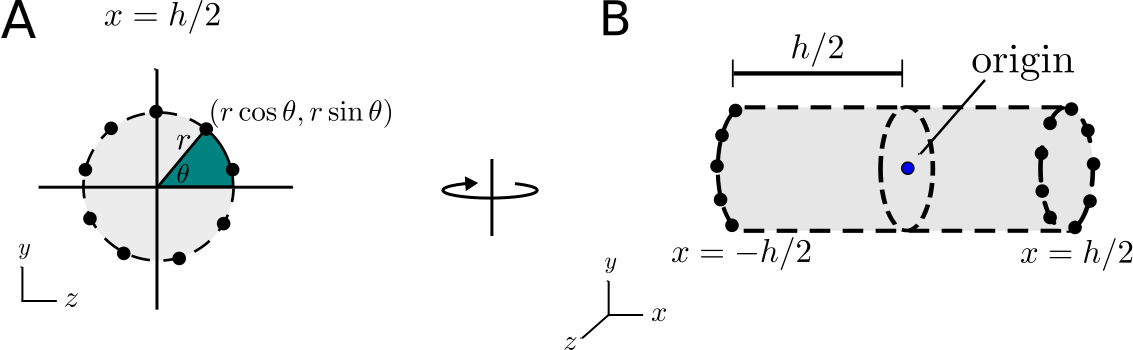
\includegraphics[width=1\textwidth]{figures/saxs/cylinder_implementation.pdf}
    \caption{Implementation of the cylindrical sample geometry in RADDOSE-3D given user defined diameter, $d$ and height $h$. (A) evenly spaced points around a circle are generated given the radius $r = d/2$ of the circular cross-section. RADDOSE-3D defaults to 32 points. (B) In three dimensions the points represent the circles at each end of the cylinder. The connectivity of these vertices is hard-coded into the RADDOSE-3D source code.}
    \label{fig:Cylindrical implementation}
\end{figure}

The cylindrical implementation is graphically depicted in Figure~\ref{fig:Cylindrical implementation}.
First the points around a circle are generated using the user defined diameter of the circular cross section.
RADDOSE-3D uses 32 points around the circle by default no matter the dimensions that are entered.
The points are evenly spaced around the circle with $y, z$ coordinates $(r \cos \theta, r \sin \theta)$.
The angle (in radians) between any two consecutive points is $2 \pi / 32$.
A cylinder can be defined by the circles at either of shape so this is done using the final coordinate $x$.
Depending on which end the point is on it'll have coordinates $(x, y, z) = (-h/2, r \cos \theta, r \sin \theta)$ or $(x, y, z) = (h/2, r \cos \theta, r \sin \theta)$.
Note that this means the origin of the system is at the very centre of the cylinder.

Regardless of the dimensions of the cylinder, the connectivity of the vertices remains the same (because the number of vertices is constant).
Therefore the connectivity has been hard-coded into RADDOSE-3D.
It will only ever need to be changed if the number of points is changed.
However this parameter is not exposed to the user and hence it would only change if a developer changed the source code.

The geometry for the cylinder sample implementation is rotated by $90^{\circ}$ about the $y$ axis as defined in Figure~\ref{fig:Cylindrical implementation}.
This means that the beam would irradiate the sample along the $x$-axis (or directly into the page looking at Figure~\ref{fig:Cylindrical implementation} A).
In a typical SAXS experiments the beam direction is along the $z$-axis (i.e. perpendicular to the axial dimension of the cylinder).
So whenever the user specifies a SAXS experiment in RADDOSE-3D the sample (it does not have to be cylindrical) is rotated by an additional $90^{\circ}$ to angle which the user specifies as the initial orientation of the sample to the beam.
This is done because it is likely to be the most common scenario for a SAXS experiment (if the experimental geometry is non-standard then the user would have to take a lot of care to ensure that the geometric parameters provided to RADDOSE-3D are correct).

\subsection{Determining the sample composition}
\label{sub:Determining the sample composition}
Knowledge of the atomic composition of the sample is necessary to be able to calculate the absorbed dose upon X-ray irradiation.
This is because the overall absorption coefficient of the sample is calculated from the individual atomic absorption coefficients.
In MX the crystal composition is calculated from the contents of the unit cell.
This is not possible in SAXS because the sample is in a liquid form as opposed to a crystalline form so it does not make sense for the user to specify contents of the unit cell.
Instead the user should know the concentration of the protein in the sample in units of milligrams per millilitre (mg/ml).
So the approach to determine the overall sample composition is to work out the atomic composition in a given volume of liquid given the protein concentration and knowledge of the composition of the buffer solution.

First the molarity of the solution is calculated as using the formula
\begin{equation}
    \text{Molarity (moles/litre)} = \f{\text{sample concentration (grams/litre)}}{\text{molecular mass (grams/mole)}}.
\end{equation}
If the sequence file is given for the protein (the sample could also contain DNA and RNA) then the molecular mass can be determined accurately from each residue in the file, otherwise an average molecular weight is used for each residue (110 daltons for protein residues, 339.5 daltons for RNA residues and 327 daltons for DNA residues) and the user has to specify the type and number of residues for the sample.

Secondly the a suitable volume needs to be specified to calculate the atomic composition. By suitable it means that volume should be large enough to contain at least one complete molecule.
By default this volume is defined to be 1000 Angstroms cubed but this can be changed by the user by specifying the length, width and height dimensions of the volume in the input file using the \textit{unit cell} input keyword.

The number of monomers/molecules in the volume can then be calculated by multiplying the molarity by the volume (converted to litres) and by Avogadro's number ($N_A = 6.022 \times 10^{23} mol^{−1}$) and then rounded to the nearest integer.
The absorption coefficient can then be calculated in the usual way as is described in \cite{pait2009}.
If there is less than 1 molecule in the volume then this is flagged up and the user is advised to increase the volume.

\subsection{Attenuation of X-ray flux due to capillary}
\label{sub:Attenuation of X-ray flux due to capillary}
In a typical MX experiment a crystal is exposed directly to the X-ray beam.
In contrast, samples from SAXS experiments are held inside a capillary.
This means that the attenuation of the X-ray flux due to the capillary needs to be taken into account before calculating the absorbed dose in the sample.
